\chapter{क्रिस्टलिकी और एक्स-किरण विवर्तन}\label{ch:b3:x-ray-diffraction}

1912 में कॉपर सल्फ़ेट के एक क्रिस्टल से होकर भेजे गए एक्स-किरणों के पुंज ने
फ़ोटोग्राफ़ी प्लेट पर तीक्ष्ण धब्बों का एक प्रतिरूप छोड़ा: क्रिस्टल एक्स-किरणों को उसी तरह
विवर्तित करते हैं जैसे ग्रेटिंग प्रकाश को, क्योंकि उनके परमाणुओं के बीच की दूरियाँ
एक्स-किरण तरंगदैर्घ्य के तुल्य होती हैं। एक वर्ष बाद विलियम लॉरेंस ब्रैग ने, जो तब
विद्यार्थी थे, ऐसे प्रतिरूपों से सैंधव लवण की संरचना पढ़ी --- और दिखाया कि
इस ठोस में \ce{NaCl} अणु होते ही नहीं, केवल एक जालक होता है जिसमें हर आयन के
दूसरे प्रकार के छह पड़ोसी होते हैं। प्रथम वर्ष के खंड में और इस पुस्तक में उद्धृत
हर क्रिस्टल संरचना इसी प्रकार ज्ञात की गई थी। यह अध्याय जालकों की और उनकी
सममिति की ज्यामिति, विवर्तन का प्रतिबंध, कोष्ठिका की सामग्री प्रकट करने वाली
तीव्रताएँ, और हर प्रयोगशाला में प्रयुक्त चूर्ण तथा
एकल-क्रिस्टल विधियाँ देता है।

\begin{recall}
प्रथम वर्ष के खंड ने क्रिस्टलों का वर्णन नोडों के जालक, एक मोटिफ़ और एक एकक
कोष्ठिका तथा उसके जालक प्राचलों से किया; कोष्ठिका की बहुकता गिनी;
फलक-केंद्रित और अंतःकेंद्रित घनीय तथा षट्कोणीय निविड़ संकुलित
संरचनाएँ, और सैंधव लवण, सीज़ियम क्लोराइड, ज़िंक ब्लेंड और फ़्लुओराइट
प्रकार बनाए; और कोष्ठिका से घनत्व परिकलित किया। \Cref{ch:b3:point-groups} ने
\omterm{def:b3:point-groups:operation}{सममिति संक्रियाएँ} और \omterm{def:b3:point-groups:point-group}{बिंदु समूह} परिभाषित किए।
\end{recall}

\begin{omfigure}
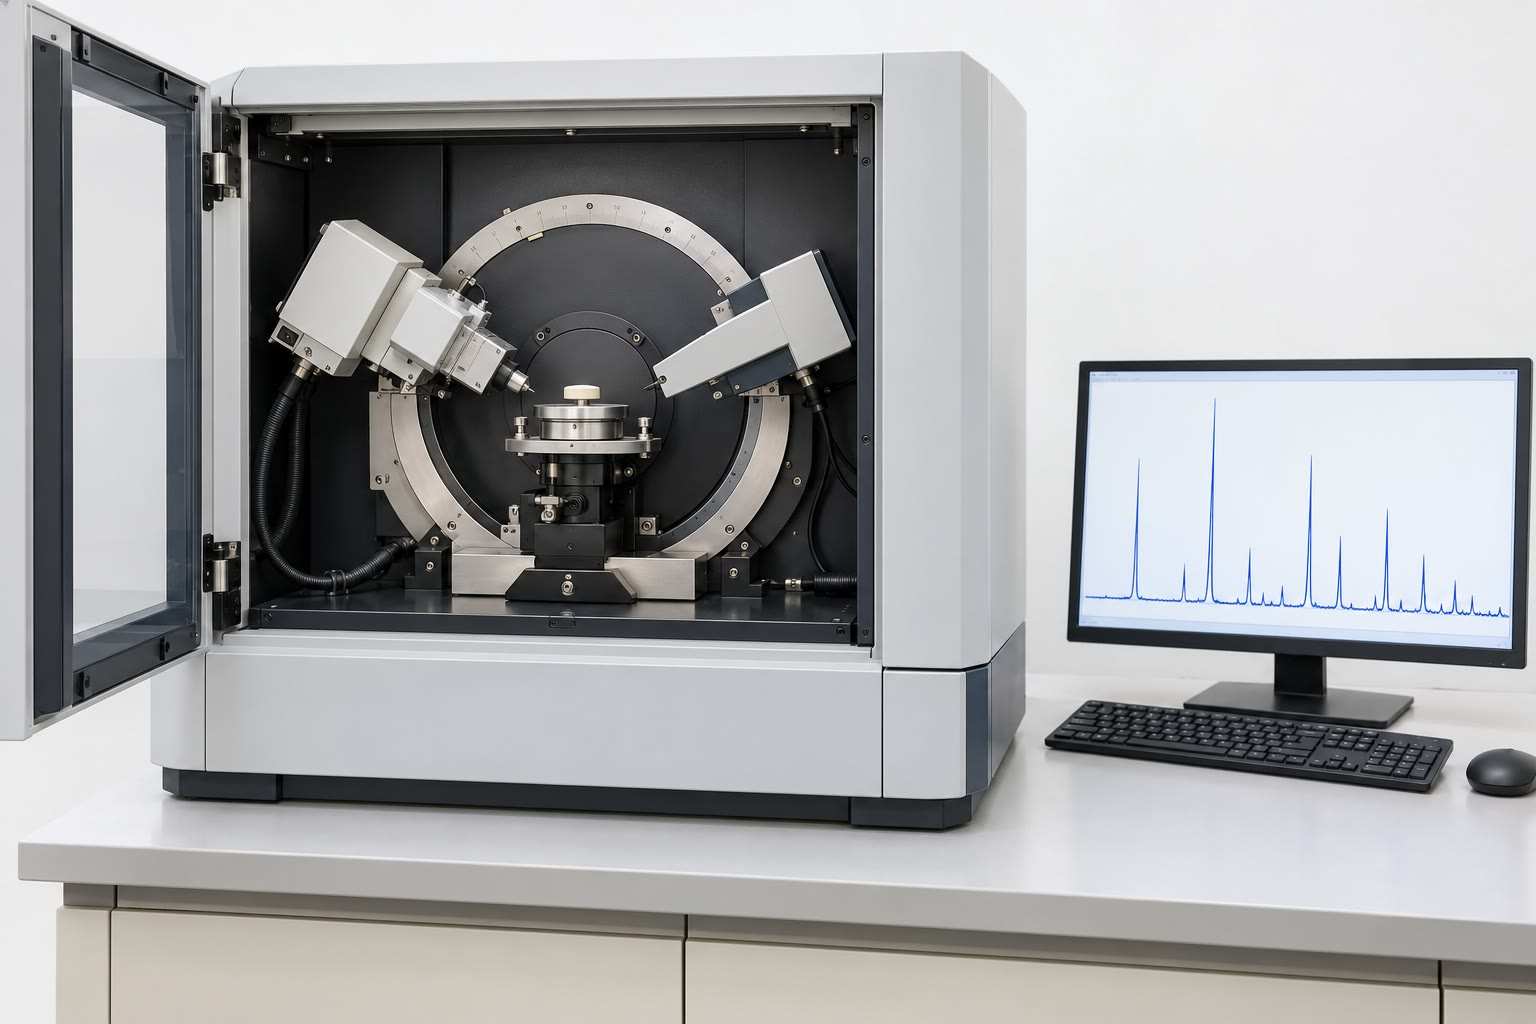
\includegraphics[width=0.6\linewidth]{images/book4/ai/b3-09-diffractometer.jpg}

{\small एक बेंच-शीर्ष चूर्ण विवर्तनमापी: एक्स-किरण नलिका और संसूचक
समतल नमूने के चारों ओर एक वृत्त पर घूमते हैं।}
\end{omfigure}

\section{क्रिस्टल तंत्र और ब्रावे जालक}

किसी जालक की केवल वही \omterm{def:b3:point-groups:operation}{सममिति संक्रियाएँ} हो सकती हैं जो जालक को स्वयं पर प्रतिचित्रित करें।
यह उन्हें कड़ाई से सीमित कर देता है।

\begin{theorem}[क्रिस्टलिकीय प्रतिबंध]\label{thm:b3:x-ray-diffraction:restriction}
किसी जालक के साथ संगत घूर्णन अक्ष केवल कोटि 1, 2, 3, 4 और 6 के होते हैं।
\end{theorem}

\begin{proof}
जालक सदिशों के आधार में सममिति घूर्णन जालक सदिशों को जालक सदिशों पर
प्रतिचित्रित करता है, अतः उसके आव्यूह की प्रविष्टियाँ पूर्णांक हैं और अनुरेख भी पूर्णांक है।
अनुरेख आधार पर निर्भर नहीं करता; अक्ष के अनुदिश $z$ वाले प्रसामान्य-लांबिक आधार में
यह $1 + 2\cos\theta$ है। अतः $2\cos\theta$, $-2$ और 2 के बीच एक पूर्णांक है:
$\cos\theta \in \{-1, -\frac12, 0, \frac12, 1\}$, $\theta = 180^\circ, 120^\circ, 90^\circ,
60^\circ, 0^\circ$: कोटियाँ 2, 3, 4, 6, 1। पंचगुण अक्ष असंभव है।
\end{proof}

\begin{definition}[क्रिस्टल तंत्र, ब्रावे जालक, जालक केंद्रण]\label{def:b3:x-ray-diffraction:crystal-system}
जालकों को उनकी सममिति के अनुसार सात \emph{क्रिस्टल
तंत्रों}\index{क्रिस्टल तंत्र} में समूहित किया जाता है (त्रिनताक्ष, एकनताक्ष, विषमलंबाक्ष, चतुष्कोणीय,
त्रिकोणीय, षट्कोणीय, घनीय)। कोई कोष्ठिका जालक नोड केवल अपने कोनों पर रख सकती है
(आद्य, P) या अपने केंद्र पर भी (अंतःकेंद्रित, I), सभी फलकों के केंद्रों पर
(फलक-केंद्रित, F) या फलकों के एक युग्म के केंद्रों पर (आधार-केंद्रित, C), या
काय-विकर्ण के अनुदिश (त्रिसमनताक्ष, R): यही उसका \emph{जालक
केंद्रण}\index{जालक केंद्रण} है। किसी तंत्र और किसी केंद्रण के 14 भिन्न संयोजन
\emph{ब्रावे जालक}\index{ब्रावे जालक} हैं।
\end{definition}

\begin{center}\small
\begin{tabular}{lll}
\hline
तंत्र & कोष्ठिका प्रतिबंध & केंद्रण \\ \hline
त्रिनताक्ष & कोई नहीं & P \\
एकनताक्ष & $\alpha = \gamma = 90^\circ$ & P, C \\
विषमलंबाक्ष & $\alpha = \beta = \gamma = 90^\circ$ & P, C, I, F \\
चतुष्कोणीय & $a = b$, सभी कोण $90^\circ$ & P, I \\
त्रिकोणीय & $a = b = c$, $\alpha = \beta = \gamma \ne 90^\circ$ (त्रिसमनताक्ष अक्ष) & R \\
षट्कोणीय & $a = b$, $\alpha = \beta = 90^\circ$, $\gamma = 120^\circ$ & P \\
घनीय & $a = b = c$, सभी कोण $90^\circ$ & P, I, F \\ \hline
\end{tabular}
\end{center}

\begin{omfigure}
\tdplotsetmaincoords{60}{100}
\begin{tikzpicture}[tdplot_main_coords, scale=1.25, font=\small]
  \foreach \s/\lab in {0/{घनीय P}, 3.0/{घनीय I}, 6.0/{घनीय F}}{
    \begin{scope}[xshift=\s cm]
      \pic[transform shape] {omcubeo={1.6}};
      \foreach \x in {0,1.6}{\foreach \y in {0,1.6}{\foreach \z in {0,1.6}{\node[cellA=2.6mm] at (\x,\y,\z) {};}}}
      \node[anchor=north] at (0.8,0.8,-0.62) {\lab};
    \end{scope}}
  \begin{scope}[xshift=3.0cm]
    \node[cellB=2.6mm] at (0.8,0.8,0.8) {};
  \end{scope}
  \begin{scope}[xshift=6.0cm]
    \foreach \p in {(0.8,0.8,0),(0.8,0.8,1.6),(0.8,0,0.8),(0.8,1.6,0.8),(0,0.8,0.8),(1.6,0.8,0.8)}{\node[cellB=2.6mm] at \p {};}
  \end{scope}
\end{tikzpicture}

{\small तीन घनीय \omterm{def:b3:x-ray-diffraction:crystal-system}{ब्रावे जालक}: आद्य (कोनों पर नोड),
अंतःकेंद्रित (साथ में केंद्र, लाल) और फलक-केंद्रित (साथ में छह फलक-केंद्र,
लाल)। उनकी कोष्ठिकाओं में 1, 2 और 4 नोड होते हैं।}
\end{omfigure}

\section{जालक तल और व्युत्क्रम जालक}

\begin{definition}[जालक तल, मिलर सूचकांक, अंतरतलीय दूरी]\label{def:b3:x-ray-diffraction:miller}
\emph{जालक तल}\index{जालक तल} कम से कम तीन असंरेख नोडों से होकर
जाने वाला तल है; वह समांतर, समदूरस्थ तलों के ऐसे कुल का सदस्य है
जिनमें हर नोड समाहित है। यदि कुल का मूलबिंदु के निकटतम तल
अक्षों को $a/h$, $b/k$, $c/l$ पर काटता है, तो उभयनिष्ठ गुणनखंड रहित पूर्णांक $(hkl)$
उसके \emph{मिलर सूचकांक}\index{मिलर सूचकांक} हैं (किसी अक्ष के समांतर तल के लिए
सूचकांक 0)। सन्निकट तलों के बीच की दूरी
\emph{अंतरतलीय दूरी}\index{अंतरतलीय दूरी} $d_{hkl}$ है।
\end{definition}

\begin{proposition}[लांबिक कोष्ठिकाओं में दूरियाँ]\label{prop:b3:x-ray-diffraction:spacing}
विषमलंबाक्ष कोष्ठिका के लिए $\dfrac{1}{d_{hkl}^2} = \dfrac{h^2}{a^2} + \dfrac{k^2}{b^2} +
\dfrac{l^2}{c^2}$; घनीय कोष्ठिका के लिए $d_{hkl} = a/\sqrt{h^2 + k^2 + l^2}$।
\end{proposition}

\begin{proof}
तल $hx/a + ky/b + lz/c = 1$ का अभिलंब सदिश $\mathbf n = (h/a, k/b, l/c)$ है
और वह मूलबिंदु से दूरी $1/|\mathbf n|$ पर है; मूलबिंदु से होकर जाने वाला समांतर तल
कुल का सदस्य है, अतः $d = 1/|\mathbf n|$।
\end{proof}

\begin{definition}[व्युत्क्रम जालक]\label{def:b3:x-ray-diffraction:reciprocal}
आधार सदिशों $\mathbf a$, $\mathbf b$, $\mathbf c$ और कोष्ठिका आयतन $V$ वाले जालक के लिए
\emph{व्युत्क्रम जालक}\index{व्युत्क्रम जालक} के आधार सदिश
$\mathbf a^* = (\mathbf b\times\mathbf c)/V$, $\mathbf b^* = (\mathbf c\times\mathbf a)/V$,
$\mathbf c^* = (\mathbf a\times\mathbf b)/V$ हैं, ताकि $\mathbf a\cdot\mathbf a^* = 1$ और
$\mathbf a\cdot\mathbf b^* = 0$। उसका नोड $\mathbf G_{hkl} = h\mathbf a^* + k\mathbf b^* + l\mathbf c^*$
तलों $(hkl)$ के लंबवत है, और $|\mathbf G_{hkl}| = 1/d_{hkl}$।
\end{definition}

\section{विवर्तन}

\begin{theorem}[ब्रैग का नियम]\label{thm:b3:x-ray-diffraction:bragg}
तरंगदैर्घ्य $\lambda$ की एक्स-किरणें दूरी $d$ वाले तलों के किसी कुल से
केवल उन स्पर्शी कोणों $\theta$ पर परावर्तित होती हैं जो इसे संतुष्ट करते हैं:
\[
2d\sin\theta = n\lambda, \qquad n = 1, 2, \dots,
\]
यही \emph{ब्रैग का नियम}\index{ब्रैग का नियम} है। कोटि $n$ को परावर्तन को
$(nh\,nk\,nl)$ लिखकर, दूरी $d/n$ के साथ, समाहित कर लिया जाता है।
\end{theorem}

\begin{proof}
दो सन्निकट तलों द्वारा प्रकीर्णित किरणों में, आपतन और परावर्तन के समान कोणों
$\theta$ पर, पथ-अंतर $2d\sin\theta$ होता है (निचले तल से होकर जाने वाले अभिलंब के
दोनों ओर के दो खंड)। जब यह अंतर तरंगदैर्घ्यों की पूर्ण संख्या हो तब वे परस्पर
सुदृढ़ होती हैं; लाखों तलों के साथ कोई भी अन्य कोण ऐसी किरणें देता है
जो युग्मों में निरस्त हो जाती हैं।
\end{proof}

\begin{omfigure}
\begin{tikzpicture}[font=\small, >=Stealth]
  \foreach \y in {0,-1.1}{\draw[thick] (-0.4,\y) -- (7.4,\y);}
  \foreach \x in {0,1.4,...,7.0}{\fill (\x,0) circle (1.5pt) (\x,-1.1) circle (1.5pt);}
  \draw[->, omDef, thick] (0.2,1.75) -- (2.8,0);
  \draw[->, omDef, thick] (2.8,0) -- (5.4,1.75);
  \draw[->, omDef, thick] (-1.43,1.75) -- (2.8,-1.1);
  \draw[->, omDef, thick] (2.8,-1.1) -- (7.03,1.75);
  \draw[densely dashed] (2.8,0) -- (2.8,-1.1);
  \draw[omThm, thick] (2.8,0) -- (2.18,-0.68) (2.8,0) -- (3.42,-0.68);
  \draw[omThm, very thick] (2.18,-0.68) -- (2.8,-1.1) -- (3.42,-0.68);
  \draw (1.8,0) arc[start angle=180, end angle=213.9, radius=1.0];
  \node[anchor=east] at (1.85,-0.2) {$\theta$};
  \draw[<->] (7.7,0) -- (7.7,-1.1) node[midway, right] {$d$};
  \node[omThm, anchor=north] at (2.8,-1.2) {पथ-अंतर $2d\sin\theta$};
\end{tikzpicture}

{\small ब्रैग की रचना। सन्निकट तलों द्वारा परावर्तित किरणें दो लाल खंडों जितनी,
हर एक $d\sin\theta$, अधिक दूरी तय करती हैं; तरंगें तब सुदृढ़ होती हैं जब
$2d\sin\theta$ तरंगदैर्घ्यों की पूर्ण संख्या हो।}
\end{omfigure}

\begin{proposition}[लाउए प्रतिबंध]\label{prop:b3:x-ray-diffraction:laue}
आपतित और प्रकीर्णित तरंग सदिशों $\mathbf k$ और $\mathbf k'$ के साथ, जिनकी लंबाई
$1/\lambda$ है, विवर्तन तब होता है जब $\mathbf k' - \mathbf k = \mathbf G_{hkl}$, जो
\omterm{def:b3:x-ray-diffraction:reciprocal}{व्युत्क्रम जालक} का एक सदिश है; यह \omterm{thm:b3:x-ray-diffraction:bragg}{ब्रैग के नियम} के तुल्य है।
\end{proposition}

\begin{proof}
जालक सदिश $\mathbf R$ से अलग दो नोडों द्वारा प्रकीर्णित तरंगों में कला-अंतर
$2\pi(\mathbf k' - \mathbf k)\cdot\mathbf R$ है; वे सभी सुदृढ़ होती हैं यदि यह $2\pi$ का गुणज हो,
हर $\mathbf R$ के लिए, अर्थात् यदि $\mathbf k' - \mathbf k$ \omterm{def:b3:x-ray-diffraction:reciprocal}{व्युत्क्रम जालक} में हो
(परिभाषा $\mathbf a\cdot\mathbf a^* = 1$, $\mathbf a\cdot\mathbf b^* = 0$\dots{} से)। प्रत्यास्थ प्रकीर्णन के लिए
$|\mathbf k| = |\mathbf k'|$ और $|\mathbf k' - \mathbf k| = 2\sin\theta/\lambda$, जहाँ $2\theta$ उनके बीच
का कोण है; $|\mathbf G| = 1/d$ के साथ यह $2d\sin\theta = \lambda$ है, और $\mathbf G$
परावर्तक तलों के अभिलंब है।
\end{proof}

\begin{definition}[एवाल्ड गोला]\label{def:b3:x-ray-diffraction:ewald}
\emph{एवाल्ड गोले}\index{एवाल्ड गोला} की त्रिज्या $1/\lambda$ है और वह
\omterm{def:b3:x-ray-diffraction:reciprocal}{व्युत्क्रम जालक} के मूलबिंदु से होकर जाता है, उसका केंद्र मूलबिंदु से $-\mathbf k$ पर है; जब भी
कोई व्युत्क्रम-जालक नोड उस पर स्थित होता है, परावर्तन होता है।
\end{definition}

\begin{omfigure}
\begin{tikzpicture}[font=\small, >=Stealth, scale=0.9]
  \foreach \i in {-2,...,4}{\foreach \j in {-2,...,2}{\fill[black!60] (\i*1.0,\j*0.75) circle (1.3pt);}}
  \node[anchor=north east] at (0,0) {$O$};
  \draw[omDef] (-1.625,0.0) circle (1.625);
  \draw[->, omDef, thick] (-1.625,0) -- (0,0) node[midway, below] {$\mathbf k$};
  \draw[->, omThm, thick] (-1.625,0) -- (-1.0,1.5);
  \node[omThm, anchor=east] at (-1.4,0.85) {$\mathbf k'$};
  \draw[->, black, very thick] (0,0) -- (-1.0,1.5) node[pos=0.3, left] {$\mathbf G$};
  \node[anchor=north] at (-1.625,-1.75) {एवाल्ड गोला, त्रिज्या $1/\lambda$};
  \draw[<->] (4.6,0) -- (4.6,0.75) node[midway, right] {$b^*$};
  \draw[<->] (3,-1.85) -- (4,-1.85) node[midway, below] {$a^*$};
\end{tikzpicture}

{\small दो विमाओं में एवाल्ड रचना (वृत्त \omterm{def:b3:x-ray-diffraction:reciprocal}{व्युत्क्रम जालक} के
मूलबिंदु $O$ से होकर जाता है)। वृत्त पर स्थित नोड $\mathbf G$ एक
विवर्तित पुंज $\mathbf k' = \mathbf k + \mathbf G$ देता है। यहाँ वृत्त, जिसकी त्रिज्या चित्र के लिए
चुनी गई है, नोड $(-1, 2)$ से होकर जाता है।}
\end{omfigure}

\section{तीव्रताएँ और सममिति}

\omterm{thm:b3:x-ray-diffraction:bragg}{ब्रैग का नियम} विवर्तित पुंजों की दिशाएँ देता है, जो केवल
जालक पर निर्भर करती हैं; उनकी तीव्रताएँ इस पर निर्भर करती हैं कि कोष्ठिका में क्या है।

\begin{definition}[परमाणु प्रकीर्णन गुणक, संरचना गुणक]\label{def:b3:x-ray-diffraction:structure-factor}
किसी परमाणु का \emph{परमाणु प्रकीर्णन गुणक}\index{परमाणु प्रकीर्णन गुणक} $f_j$
वह आयाम है जिसे वह प्रकीर्णित करता है, एक इलेक्ट्रॉन के आयाम की इकाइयों में; अग्र दिशा में यह
उसके इलेक्ट्रॉनों की संख्या के बराबर है और ऊँचे कोणों पर घटता जाता है।
परावर्तन $hkl$ का \emph{संरचना गुणक}\index{संरचना गुणक} यह है:
\[
F_{hkl} = \sum_jf_j\,\eu^{2\pi\iu(hx_j + ky_j + lz_j)},
\]
जो कोष्ठिका के उन परमाणुओं पर जोड़ा गया है जो भिन्नात्मक निर्देशांकों $(x_j, y_j, z_j)$ पर हैं।
\end{definition}

\begin{proposition}[तीव्रता]\label{prop:b3:x-ray-diffraction:intensity}
किसी परावर्तन की तीव्रता $|F_{hkl}|^2$ के समानुपाती है।
\end{proposition}

\begin{proof}[आंशिक उपपत्ति]
परमाणु $j$, $\mathbf r_j = x_j\mathbf a + y_j\mathbf b + z_j\mathbf c$ पर स्थित है; किसी परावर्तन के लिए
$(\mathbf k' - \mathbf k)\cdot\mathbf r_j = hx_j + ky_j + lz_j$, अतः उसकी तरंग की कला
मूलबिंदु पर स्थित परमाणु के सापेक्ष $2\pi(hx_j + ky_j + lz_j)$ है, और आयाम $f_j$:
कोष्ठिका योग $F_{hkl}$ प्रकीर्णित करती है, और हर कोष्ठिका वही। तीव्रता किसी आयाम के
मापांक का वर्ग होती है। बहु-प्रकीर्णन की उपेक्षा की जा सकती है
(शुद्धगतिक सन्निकटन), यह स्वीकार किया गया है।
\end{proof}

\begin{definition}[क्रमबद्ध अनुपस्थिति]\label{def:b3:x-ray-diffraction:absence}
\emph{क्रमबद्ध अनुपस्थिति}\index{क्रमबद्ध अनुपस्थिति} ऐसा परावर्तन है जिसका
\omterm{def:b3:x-ray-diffraction:structure-factor}{संरचना गुणक} दिए हुए \omterm{def:b3:x-ray-diffraction:crystal-system}{जालक केंद्रण} या सममिति वाले हर क्रिस्टल के लिए
लुप्त होता है, चाहे उसके परमाणु कोई भी हों।
\end{definition}

\begin{proposition}[केंद्रित जालकों की अनुपस्थितियाँ]\label{prop:b3:x-ray-diffraction:absences}
अंतःकेंद्रित जालक में $h + k + l$ विषम वाले परावर्तन अनुपस्थित होते हैं;
फलक-केंद्रित जालक में मिश्रित समता वाले $h$, $k$, $l$ के परावर्तन अनुपस्थित होते हैं।
\end{proposition}

\begin{proof}
I केंद्रण: $(x,y,z)$ पर स्थित हर परमाणु की एक प्रति $(x + \frac12, y + \frac12, z + \frac12)$ पर है,
जिसका कला गुणक $\eu^{\iu\pi(h+k+l)} = (-1)^{h+k+l}$ से भिन्न है: $F = (1 +
(-1)^{h+k+l})F'$। F केंद्रण: तीन फलक-केंद्रों पर प्रतियाँ गुणक $1 +
(-1)^{h+k} + (-1)^{h+l} + (-1)^{k+l}$ देती हैं, जो 4 के बराबर है यदि $h$, $k$, $l$ सभी सम या सभी विषम हों,
और अन्यथा 0।
\end{proof}

\begin{example}[सैंधव लवण और सिल्वाइट]\label{ex:b3:x-ray-diffraction:nacl-kcl}
% ledger: lat:NaCl, lat:KCl
सैंधव-लवण संरचना में धनायन $(0,0,0)$ पर और ऋणायन $(\frac12,0,0)$ पर, हर एक
F स्थानांतरणों के साथ: अमिश्रित सूचकांकों के लिए $F_{hkl} = 4[f_+ + f_-(-1)^{h+k+l}]$।
\ce{NaCl} के लिए $f(\ce{Na+}) \approx 10$ और $f(\ce{Cl-}) \approx 18$: सभी-विषम परावर्तन
(111), (311) दुर्बल हैं परंतु उपस्थित। \ce{KCl} के लिए \ce{K+} और \ce{Cl-} दोनों के 18
इलेक्ट्रॉन हैं: सभी-विषम परावर्तन लगभग लुप्त हो जाते हैं, और प्रतिरूप आधी कोष्ठिका-कोर वाले
आद्य घनीय जालक जैसा दिखता है (नीचे का चित्र)।
\end{example}

\begin{omfigure}
\begin{tikzpicture}
\begin{axis}[name=salts, width=0.95\linewidth, height=5.2cm, xmin=20, xmax=90,
  ymin=0, ymax=2.55, ytick=\empty, axis x line=bottom, axis y line=none,
  xlabel={$2\theta$ / अंश (Cu K$\alpha_1$)}, tick label style={font=\small},
  label style={font=\small}]
\addplot[omDef, thin] table[x=tt, y expr=\thisrow{NaCl}+1.35] {figdata/out/bachelor-3-xrd-powder-salts.dat};
\addplot[omThm, thin] table[x=tt, y=KCl] {figdata/out/bachelor-3-xrd-powder-salts.dat};
\node[font=\small, omDef, anchor=west] at (axis cs:79,1.9) {\ce{NaCl}};
\node[font=\small, omThm, anchor=west] at (axis cs:77,0.55) {\ce{KCl}};
\node[font=\scriptsize, anchor=south] at (axis cs:27.36,1.52) {111};
\node[font=\scriptsize, anchor=west] at (axis cs:32.1,2.25) {200};
\node[font=\scriptsize, anchor=west] at (axis cs:28.8,0.9) {200};
\node[font=\scriptsize, anchor=west] at (axis cs:41.0,0.85) {220};
\end{axis}
\end{tikzpicture}

\begin{tikzpicture}
\begin{axis}[name=met, width=0.62\linewidth, height=4.4cm, xmin=35, xmax=100,
  ymin=0, ymax=2.35, ytick=\empty, axis x line=bottom, axis y line=none,
  xlabel={$2\theta$ / अंश}, tick label style={font=\small}, label style={font=\small}]
\addplot[omDef, thin] table[x=tt, y expr=\thisrow{Cu}+1.2] {figdata/out/bachelor-3-xrd-powder-metals.dat};
\addplot[omThm, thin] table[x=tt, y=W] {figdata/out/bachelor-3-xrd-powder-metals.dat};
\node[font=\small, omDef, anchor=west] at (axis cs:55,1.5) {Cu (F)};
\node[font=\small, omThm, anchor=west] at (axis cs:44,0.4) {W (I)};
\end{axis}
\begin{axis}[at={(met.east)}, anchor=west, xshift=0.7cm, width=0.36\linewidth, height=4.4cm,
  xmin=29.7, xmax=33.7, ymin=0, ymax=1.1, ytick=\empty, axis x line=bottom,
  axis y line=none, xlabel={$2\theta$ / अंश}, tick label style={font=\small},
  label style={font=\small}, title={\small शेरर}]
\addplot[black, thick] table[x=tt, y=L200] {figdata/out/bachelor-3-xrd-powder-scherrer.dat};
\addplot[omDef, thick] table[x=tt, y=L50] {figdata/out/bachelor-3-xrd-powder-scherrer.dat};
\addplot[omThm, thick] table[x=tt, y=L10] {figdata/out/bachelor-3-xrd-powder-scherrer.dat};
\end{axis}
\end{tikzpicture}

{\small परिकलित चूर्ण प्रतिरूप (Cu K$\alpha_1$; प्रकीर्णन गुणक
इलेक्ट्रॉनों की संख्याओं के बराबर लिए गए हैं, अतः केवल अनुपस्थितियाँ और तीव्रता की
व्यापक प्रवृत्तियाँ अर्थपूर्ण हैं)। ऊपर: \ce{NaCl} और \ce{KCl}; \ce{KCl} की सभी-विषम रेखाएँ
लुप्त हो जाती हैं। नीचे बाएँ: कॉपर (F) में (111), (200), (220), (311)\dots{} दिखते हैं; टंगस्टन
(I) में (110), (200), (211)\dots। नीचे दाएँ: \ce{NaCl} की (200) रेखा,
200 (काला), 50 (नीला) और 10 nm (लाल) के क्रिस्टलकों के लिए: छोटे क्रिस्टल
चौड़ी रेखाएँ देते हैं।}
\end{omfigure}

\begin{proposition}[फ़्रीडेल का नियम]\label{prop:b3:x-ray-diffraction:friedel}
असामान्य प्रकीर्णन की अनुपस्थिति में $|F_{hkl}| = |F_{\bar h\bar k\bar l}|$: विवर्तन
प्रतिरूप केंद्रसममित दिखता है, तब भी जब क्रिस्टल केंद्रसममित न हो।
\end{proposition}

\begin{proof}
वास्तविक $f_j$ के साथ $F_{\bar h\bar k\bar l} = \sum f_j\eu^{-2\pi\iu(\dots)} = F_{hkl}^*$, जिसका
मापांक वही है।
\end{proof}

किसी घूर्णन या परावर्तन को जालक स्थानांतरण के किसी अंश के साथ संयोजित करने वाले
\omterm{def:b3:point-groups:operation}{सममिति तत्व} केवल क्रिस्टलों में होते हैं।

\begin{definition}[पेंच अक्ष, सर्पी तल, आकाशी समूह]\label{def:b3:x-ray-diffraction:space-group}
\emph{पेंच अक्ष}\index{पेंच अक्ष} $n_p$, $2\pi/n$ के घूर्णन को
अक्ष के अनुदिश जालक पुनरावृत्ति के $p/n$ के स्थानांतरण से संयोजित करता है ($2_1$: आधा घुमाव और
आधी कोष्ठिका)। \emph{सर्पी तल}\index{सर्पी तल} किसी परावर्तन को
तल के समांतर आधे जालक सदिश के स्थानांतरण से संयोजित करता है ($a$, $b$, $c$ सर्पण)।
किसी क्रिस्टल की सभी \omterm{def:b3:point-groups:operation}{सममिति संक्रियाओं} का समूह, स्थानांतरणों सहित,
उसका \emph{आकाशी समूह}\index{आकाशी समूह} है: ऐसे 230 हैं। उसका सबसे छोटा भाग
जिससे संक्रियाएँ पूरा क्रिस्टल उत्पन्न करती हैं,
\emph{असममित इकाई}\index{असममित इकाई} है। बिंदुओं का ऐसा समुच्चय जिसे संक्रियाओं का कोई
\omterm{def:b3:point-groups:class}{उपसमूह} स्वयं पर छोड़ता है, \emph{वाइकॉफ़
स्थिति}\index{वाइकॉफ़ स्थिति} है: सामान्य स्थितियों की कोई सममिति नहीं होती, विशेष
स्थितियाँ \omterm{def:b3:point-groups:operation}{सममिति तत्वों} पर स्थित होती हैं।
\end{definition}

\begin{proposition}[पेंच अक्ष से अनुपस्थितियाँ]\label{prop:b3:x-ray-diffraction:screw-absence}
$2_1$ अक्ष, $b$ के अनुदिश, परावर्तनों $0k0$ को, $k$ विषम होने पर, अनुपस्थित कर देता है।
\end{proposition}

\begin{proof}
अक्ष $(x, y, z)$ को $(-x, y + \frac12, -z)$ पर प्रतिचित्रित करता है। $h = l = 0$ के लिए दोनों परमाणुओं के
कला गुणक $\eu^{2\pi\iu ky}$ और $\eu^{2\pi\iu k(y + 1/2)} = (-1)^k\eu^{2\pi\iu ky}$ हैं: उनका योग
विषम $k$ के लिए लुप्त होता है।
\end{proof}

\begin{method}[आकाशी-समूह प्रतीक पढ़ना]\label{met:b3:x-ray-diffraction:read-space-group}
\begin{enumerate}
  \item पहला अक्षर \omterm{def:b3:x-ray-diffraction:crystal-system}{जालक केंद्रण} है (P, I, F, C, R)।
  \item अगले प्रतीक मुख्य दिशाओं के अनुदिश सममिति देते हैं;
        एकनताक्ष तंत्र के लिए एकमात्र दिशा $b$ है। भिन्न-रेखा का अर्थ है
        ``इस अक्ष के लंबवत एक तल के साथ''।
  \item \textit{P}$2_1/c$, कार्बनिक अणुओं का सबसे सामान्य \omterm{def:b3:x-ray-diffraction:space-group}{आकाशी समूह}: आद्य,
        एक $2_1$ अक्ष, $b$ के अनुदिश, और उसके लंबवत एक $c$-सर्पी तल; ये
        \omterm{def:b3:point-groups:inversion}{प्रतिलोमन केंद्र} उत्पन्न करते हैं। अनुपस्थितियाँ: $0k0$, $k$ विषम होने पर; $h0l$, $l$
        विषम होने पर।
\end{enumerate}
\end{method}

\begin{omfigure}
\begin{tikzpicture}[x=3.6cm, y=3.6cm, font=\small]
  \draw (0,0) rectangle (1,1);
  \node[anchor=north] at (0.5,-0.05) {$a \rightarrow$};
  \node[anchor=east] at (-0.05,0.5) {$b \uparrow$};
  % c-glide planes perpendicular to b at y = 1/4 and 3/4 (glide along c, normal to the page): dotted
  \draw[black, line width=1.1pt, dotted] (0,0.25) -- (1,0.25) (0,0.75) -- (1,0.75);
  % 2_1 axes parallel to b at x = 0, 1/2, 1 (height z = 1/4): lines with half-arrowheads
  \foreach \x in {0,0.5,1}{
    \draw[black, line width=1pt, {Straight Barb[left]}-{Straight Barb[left]}] (\x,0.03) -- (\x,0.97);}
  \node[font=\scriptsize, anchor=west] at (0.51,0.88) {$\tfrac14$};
  % centres of inversion at the corners, edge midpoints and centre
  \foreach \p in {(0,0),(0.5,0),(1,0),(0,0.5),(0.5,0.5),(1,0.5),(0,1),(0.5,1),(1,1)}{\pic at \p {ominv};}
  % general positions: (x,y,z), (-x,y+1/2,1/2-z), (-x,-y,-z), (x,1/2-y,1/2+z)
  \pic at (0.20,0.10) {omgenpos={$+$}{0}};
  \pic at (0.80,0.60) {omgenpos={$\tfrac12{-}$}{0}};
  \pic at (0.80,0.90) {omgenpos={$-$}{1}};
  \pic at (0.20,0.40) {omgenpos={$\tfrac12{+}$}{1}};
\end{tikzpicture}

{\small \omterm{def:b3:x-ray-diffraction:space-group}{आकाशी समूह} \textit{P}$2_1/c$, $c$ के अनुदिश देखा गया ($ab$ तल पर प्रक्षेप)।
बिंदुकित रेखाएँ: $c$-सर्पी तल, $b$ के लंबवत; अर्ध-तीर: $2_1$ \omterm{def:b3:x-ray-diffraction:space-group}{पेंच अक्ष},
$b$ के अनुदिश (ऊँचाई $z = \frac14$ पर); छोटे वृत्त: \omterm{def:b3:point-groups:inversion}{प्रतिलोमन केंद्र}। ऊँचाई $+z$ पर स्थित
एक सामान्य स्थिति तीन अन्य उत्पन्न करती है; अल्पविराम दर्पण-प्रतिबिंब
प्रति (सर्पण या प्रतिलोमन द्वारा उत्पन्न) को चिह्नित करता है; $\frac12{-}$ का अर्थ है ऊँचाई $\frac12 - z$।}
\end{omfigure}

\section{चूर्ण और एकल-क्रिस्टल विधियाँ}

\begin{definition}[चूर्ण विवर्तन प्रतिरूप]\label{def:b3:x-ray-diffraction:powder}
बारीक पिसे नमूने में सभी अभिविन्यासों के क्रिस्टलक होते हैं: तलों का हर
कुल कुछ क्रिस्टलकों को परावर्तक स्थिति में पाता है, और विवर्तित पुंज
शंकु बनाते हैं। $2\theta$ के विरुद्ध अभिलिखित तीव्रता उसका \emph{चूर्ण
विवर्तन प्रतिरूप}\index{चूर्ण विवर्तन प्रतिरूप} है, क्रिस्टलीय प्रावस्था की
एक अंगुलिछाप।
\end{definition}

\begin{method}[घनीय चूर्ण प्रतिरूप का सूचकांकन]\label{met:b3:x-ray-diffraction:index-cubic}
\begin{enumerate}
  \item हर रेखा के लिए $\sin^2\theta$ परिकलित कीजिए; घनीय क्रिस्टल के लिए $\sin^2\theta =
        (\lambda^2/4a^2)N$, जहाँ $N = h^2 + k^2 + l^2$।
  \item सबसे छोटे मान से भाग दीजिए और पूर्णांक श्रेणी खोजिए: P देता है
        $N = 1, 2, 3, 4, 5, 6, 8, \dots$ (कभी 7 नहीं); I देता है $2, 4, 6, 8, 10, \dots$; F देता है
        $3, 4, 8, 11, 12, 16, \dots$
  \item वह श्रेणी चुनिए जो सभी रेखाओं पर सटीक बैठे; तब $a = \lambda\sqrt N/(2\sin\theta)$, सबसे अच्छा
        ऊँचे कोण वाली रेखाओं से, जहाँ $\theta$ की त्रुटि सबसे कम मायने रखती है।
\end{enumerate}
\end{method}

\begin{method}[कोष्ठिका में सूत्र इकाइयों की संख्या]\label{met:b3:x-ray-diffraction:z-from-density}
एक सूत्र इकाई के मोलर द्रव्यमान $M$ और मापे गए घनत्व $\rho$ के साथ, $Z =
\rho N_Aa^3/M$ (घनीय कोष्ठिका के लिए) एक पूर्ण संख्या होनी चाहिए; यह प्रस्तावित
संरचना की परीक्षा करता है।
\end{method}

\begin{proposition}[शेरर समीकरण]\label{prop:b3:x-ray-diffraction:scherrer}
माध्य आकार $L$ के क्रिस्टलक किसी रेखा को $\beta \approx K\lambda/(L\cos\theta)$ से चौड़ा करते हैं
($2\theta$ के रेडियनों में अर्ध-अधिकतम पर पूर्ण चौड़ाई, $K \approx 0.9$)।
\end{proposition}
\admitted

लगभग \qty{100}{nm} से नीचे चौड़ीकरण मापनीय हो जाता है; शेरर
समीकरण, जो अधिक उन्नत पाठ्यक्रमों में तलों के परिमित ढेर के फ़ूरिये रूपांतर से
व्युत्पन्न किया जाता है, तब नैनोक्रिस्टलों का आकार आकलित करता है
(\cref{ch:b3:inorganic-materials})।

\begin{definition}[कला समस्या, R गुणक]\label{def:b3:x-ray-diffraction:refinement}
तीव्रताएँ $|F_{hkl}|$ देती हैं परंतु $F_{hkl}$ की कलाएँ नहीं; उनके बिना
फ़ूरिये श्रेणी के प्रतिलोमन से \omterm{def:b3:computational-chemistry:dft}{इलेक्ट्रॉन घनत्व} परिकलित नहीं किया जा सकता।
यही \emph{कला समस्या}\index{कला समस्या} है। किसी परीक्षण संरचना
को न्यूनतम वर्ग विधि से तब तक परिष्कृत किया जाता है जब तक परिकलित और प्रेक्षित मापांक मेल न खाएँ;
अवशिष्ट $R = \sum\big||F_o| - |F_c|\big|/\sum|F_o|$ उसका \emph{R
गुणक}\index{R गुणक} है --- अच्छी संरचना के लिए कुछ प्रतिशत।
\end{definition}

एकल क्रिस्टल के लिए विवर्तनमापी हज़ारों परावर्तन मापता है;
प्रत्यक्ष विधियाँ (प्रबल परावर्तनों की कलाओं के बीच सांख्यिकीय संबंध) अधिकांश छोटे
अणुओं के लिए पहला इलेक्ट्रॉन-घनत्व मानचित्र देती हैं, और
परिष्करण हर परमाणु को नैनोमीटर के कुछ हज़ारवें भाग तक स्थित कर देता है।
परिणाम CIF फ़ाइलों के रूप में मुक्त डेटाबेसों में जमा किए जाते हैं, जिनसे इस श्रृंखला
में उद्धृत जालक प्राचल लिए गए हैं।

\begin{inthelab}[एक चूर्ण मापन]
चूर्ण को अगेट खरल में पीसा जाता है, एक धारक में समतल दबाया जाता है, और
$2\theta$ में 5 से \ang{90} तक क्रमवीक्षित किया जाता है, Cu K$\alpha$ विकिरण से; एक निकेल
फ़िल्टर K$\beta$ रेखा का अधिकांश भाग हटा देता है। प्रतिरूप की तुलना किसी डेटाबेस के
संदर्भ प्रतिरूपों से की जाती है, और जालक प्राचल सिलिकॉन चूर्ण जैसे किसी
आंतरिक मानक के साथ परिष्कृत किए जाते हैं। एक्स-किरण उपकरण घिरे हुए
और अंतर्बंधित होते हैं: दरवाज़ा खुला हो तो शटर नहीं खुल सकता।
\end{inthelab}

\begin{history}[ब्रैग पिता-पुत्र, 1913]
\begin{minipage}[t]{0.72\linewidth}
मैक्स फ़ॉन लाउए ने 1912 में प्रस्तावित किया कि क्रिस्टल एक्स-किरणों को विवर्तित करते हैं, और वाल्टर फ़्रीडरिख
तथा पॉल क्निपिंग ने पहला प्रतिरूप अभिलिखित किया। बाईस वर्षीय विलियम लॉरेंस ब्रैग ने
धब्बों की व्याख्या \omterm{def:b3:x-ray-diffraction:miller}{जालक तलों} से परावर्तन के रूप में की
और, अपने पिता विलियम हेनरी ब्रैग के साथ, जिन्होंने एक्स-किरण स्पेक्ट्रममापी बनाया था,
1913 में \ce{NaCl}, \ce{KCl} और हीरे की संरचनाएँ हल कीं। पिता और पुत्र को
1915 का भौतिकी का नोबेल पुरस्कार साझा रूप से मिला।
\end{minipage}\hfill
\begin{minipage}[t]{0.22\linewidth}\vspace{0pt}
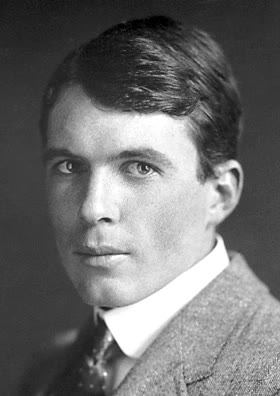
\includegraphics[width=\linewidth]{images/book4/bragg-wl.jpg}\par
{\footnotesize डब्ल्यू॰ एल॰ ब्रैग।}
\end{minipage}
\end{history}

\section{अभ्यास}

\begin{exercise}[$\star$]\label{exo:b3:x-ray-diffraction:1}
% ledger: lat:NaCl
\ce{NaCl} ($a = \qty{564.06}{pm}$) के लिए $d_{111}$, $d_{200}$ और $d_{220}$ परिकलित कीजिए।
\end{exercise}

\begin{exercise}[$\star$]\label{exo:b3:x-ray-diffraction:2}
% ledger: lat:Cu, xray:CuKa1
कॉपर FCC है, $a = \qty{361.50}{pm}$ के साथ। Cu K$\alpha_1$ ($\lambda = \qty{154.06}{pm}$) से
उसके पहले दो परावर्तनों को नाम देकर उनका $2\theta$ परिकलित कीजिए।
\end{exercise}

\begin{exercise}[$\star$]\label{exo:b3:x-ray-diffraction:3}
घनीय P, I और F जालक के लिए परावर्तनों 100, 110, 111, 200, 210, 211, 220 में से
कौन-से उपस्थित हैं?
\end{exercise}

\begin{exercise}[$\star$]\label{exo:b3:x-ray-diffraction:4}
भुजाओं $a$ और $b$ वाले द्विविमीय आयताकार जालक का व्युत्क्रम आधार दीजिए,
और पहले व्युत्क्रम नोड खींचिए।
\end{exercise}

\begin{exercise}[$\star\star$]\label{exo:b3:x-ray-diffraction:5}
% ledger: lat:W
एक धातु $2\theta = 40.27$, 58.26, 73.20, 87.01 और \ang{100.66} पर रेखाएँ
देती है, Cu K$\alpha_1$ के साथ। प्रतिरूप का सूचकांकन कीजिए, जालक का प्रकार और $a$ ज्ञात कीजिए।
\end{exercise}

\begin{exercise}[$\star\star$]\label{exo:b3:x-ray-diffraction:6}
% ledger: lat:KCl
\ce{KCl} ($a = \qty{629.29}{pm}$) के एक क्रिस्टल का मापा गया घनत्व
\qty{1.99}{g/cm^3} है (अभ्यास के आँकड़े)। $Z$ ज्ञात कीजिए।
\end{exercise}

\begin{exercise}[$\star\star$]\label{exo:b3:x-ray-diffraction:7}
\ce{NaCl} नैनोचूर्ण की (200) रेखा ($2\theta = \ang{31.70}$) \ang{0.40} चौड़ी है,
उपकरण का योगदान शून्य है। क्रिस्टलक आकार का आकलन कीजिए।
\end{exercise}

\begin{exercise}[$\star\star$]\label{exo:b3:x-ray-diffraction:8}
\ce{CsCl} में P कोष्ठिका में \ce{Cs+}, $(0,0,0)$ पर और \ce{Cl-}, $(\frac12,\frac12,\frac12)$ पर है। $f
\approx$ इलेक्ट्रॉनों की संख्या लेकर $F_{100}$ और $F_{110}$ तथा उनकी
तीव्रताओं का अनुपात (केवल \omterm{def:b3:x-ray-diffraction:structure-factor}{संरचना गुणक}) परिकलित कीजिए। \ce{CsCl} अंतःकेंद्रित क्यों नहीं है?
\end{exercise}

\begin{exercise}[$\star\star$]\label{exo:b3:x-ray-diffraction:9}
दिखाइए कि C-केंद्रित जालक ($(\frac12,\frac12,0)$ पर अतिरिक्त नोड) $h + k$ विषम वाले
परावर्तनों को अनुपस्थित कर देता है।
\end{exercise}

\begin{exercise}[$\star\star\star$]\label{exo:b3:x-ray-diffraction:10}
समझाइए कि 1980 के दशक में ऐसी मिश्रधातुओं की खोज, जिनके विवर्तन प्रतिरूप दसगुण
सममिति वाले तीक्ष्ण धब्बे दिखाते हैं, क्रिस्टलिकीय प्रतिबंध का खंडन क्यों नहीं करती,
और उसने क्रिस्टल की परिभाषा में क्या बदला।
\end{exercise}

\begin{exercise}[$\star\star\star$]\label{exo:b3:x-ray-diffraction:11}
दिखाइए कि \textit{P}$2_1/c$ में \omterm{def:b3:x-ray-diffraction:space-group}{सर्पी तल} परावर्तनों $h0l$ को, $l$
विषम होने पर, अनुपस्थित कर देता है।
\end{exercise}

\begin{exercise}[$\star\star\star$]\label{exo:b3:x-ray-diffraction:12}
शुद्ध प्रतिबिंबरूपी कभी ऐसे \omterm{def:b3:x-ray-diffraction:space-group}{आकाशी समूह} में क्रिस्टलित नहीं हो सकता जिसमें
\omterm{def:b3:point-groups:inversion}{प्रतिलोमन केंद्र}, दर्पण या \omterm{def:b3:x-ray-diffraction:space-group}{सर्पी तल} हो। क्यों? वह किस प्रकार के \omterm{def:b3:x-ray-diffraction:space-group}{आकाशी समूहों} तक
सीमित है, और उसके निरपेक्ष विन्यास के निर्धारण के लिए फ़्रीडेल के नियम का क्या
निहितार्थ है?
\end{exercise}

% keep the heading with its problem box, which fills a page by itself
\clearpage
\enlargethispage{3\baselineskip}
\section{समस्या: कौन-सा सफ़ेद चूर्ण?}

\begin{problem}[{सप्ताहांत समस्या --- किसी अज्ञात घनीय लवण का चूर्ण प्रतिरूप:
दूरियाँ, सूचकांकन, जालक प्राचल और लवण की पहचान, और
उसके क्रिस्टलकों का आकार}]
\label{pb:b3:x-ray-diffraction:1}
% ledger: xray:CuKa1, lat:NaCl, lat:KCl, lat:KBr
एक अज्ञात सफ़ेद क्रिस्टलीय चूर्ण, जिसके \ce{NaCl}, \ce{KCl} या \ce{KBr} होने का ज्ञान है,
Cu K$\alpha_1$ विकिरण ($\lambda = \qty{154.059}{pm}$) के साथ ये रेखाएँ देता है (समस्या के
आँकड़े, इस अभ्यास के लिए परिकलित):
\begin{center}\small
\begin{tabular}{lcccccc}
\hline
$2\theta$ / अंश & 28.342 & 40.512 & 50.178 & 58.632 & 66.380 & 73.692 \\
आपेक्षिक तीव्रता & 100 & 92 & 38 & 20 & 61 & 49 \\ \hline
\end{tabular}
\end{center}
20 और \ang{75} के बीच कोई अन्य रेखा नहीं दिखती। संदर्भ जालक प्राचल:
\ce{NaCl} \qty{564.06}{pm}, \ce{KCl} \qty{629.29}{pm}, \ce{KBr} \qty{658.47}{pm}। मोलर द्रव्यमान:
K 39.1, Na 23.0, Cl 35.5, Br \qty{79.9}{g/mol}।

\medskip\noindent\textbf{भाग I --- दूरियाँ।}
\begin{enumerate}
  \item पहली रेखा के लिए $\theta$ और $d$ परिकलित कीजिए।
  \item सभी रेखाओं के लिए $d$ परिकलित कीजिए।
  \item अनुपात $\sin^2\theta/\sin^2\theta_1$ परिकलित कीजिए।
  \item आपको पूर्णांकों की कौन-सी श्रेणी मिलती है?
  \item क्या यह प्रतिरूप किसी आद्य घनीय जालक का हो सकता है? किस $a$ के साथ?
  \item आद्य घनीय जालक के लिए कौन-सा पूर्णांक $N$ कभी नहीं आ सकता? क्या
        अब तक प्रतिरूप दोनों व्याख्याओं में भेद करता है?
\end{enumerate}

\medskip\noindent\textbf{भाग II --- वास्तविक जालक।}
\begin{enumerate}[resume]
  \item तीनों उम्मीदवार F जालक हैं। F श्रेणी से रेखाओं का सूचकांकन कीजिए।
  \item पहली रेखा से $a$ निकालिए।
  \item कौन-सा उम्मीदवार सटीक बैठता है?
  \item उस लवण के लिए सभी-विषम परावर्तन (111), (311) अनुपस्थित क्यों हैं?
  \item क्या \ce{NaCl} (111) दिखाएगा? \ce{KBr}?
  \item समझाइए कि भाग I की आद्य व्याख्या एक जाल क्यों है।
\end{enumerate}

\medskip\noindent\textbf{भाग III --- घनत्व और सामग्री।}
\begin{enumerate}[resume]
  \item कोष्ठिका में कितनी सूत्र इकाइयाँ हैं?
  \item कोष्ठिका से घनत्व परिकलित कीजिए।
  \item हर आयन की उपसहसंयोजन संख्या दीजिए।
  \item सबसे छोटी K--Cl दूरी परिकलित कीजिए।
  \item \ang{75} के ऊपर सबसे पहले कौन-सा परावर्तन दिखेगा?
  \item किसी प्रावस्था की पहचान के लिए तीव्रताएँ स्थितियों से कम उपयोगी क्यों हैं?
\end{enumerate}

\medskip\noindent\textbf{भाग IV --- परिष्करण और क्रिस्टलक आकार।}
\begin{enumerate}[resume]
  \item जालक प्राचल सबसे अच्छा ऊँचे कोण वाली रेखा से क्यों परिकलित होता है?
  \item (420) रेखा से $a$ परिकलित कीजिए।
  \item (420) रेखा $2\theta$ में \ang{0.25} चौड़ी है (उपकरणीय चौड़ाई
        नगण्य)। क्रिस्टलक आकार का आकलन कीजिए।
  \item क्या \qty{1}{\micro m} का क्रिस्टलक आकार रेखा को मापनीय रूप से चौड़ा करेगा?
  \item परिणाम बताइए: (420) रेखा से परिष्कृत जालक प्राचल, और
        चूर्ण की पहचान।
\end{enumerate}
\end{problem}
